\documentclass[../main.tex]{subfiles}
\begin{document}
\setchapterstyle{kao}
\setchapterpreamble[u]{\margintoc}
\chapter[Group Theory and Quantum Mechanics]{Group Theory and Quantum Mechanics\footnotemark[0]}
\labch{GT-QM}
%From 59:14
We know a lot about Lie groups and Lie algebras, at least to an introductory level. Now we want to see how these concepts enter on the stage of quantum theory and we start with quantum mechanics.
\section{Action on the state space}
First we have to consider the action of transformations, or symmetries, on the states space. Recall that in QM, the space of \textbf{pure states}\index{Pure states} is the projective space of a complex Hilbert space:
\[
S=\mathbb{P}\mathcal{H}=\left\{[\psi]:[\psi] \text{ is a ray in } \mathcal{H}\right\}
\]
The important point is that a state in QM is \textbf{not} represented by a non-zero vector in the Hilbert space but properly speaking it is represented by a ray in the Hilbert space, so two vectors which differ by a phase (e.g. $\psi$ and $-\psi$, $\psi$ and $e^{i\theta}\psi$) correspond to the same state. For many applications this is irrelevant, for example if we want to compute eigenstates and eigenvectors we assume that a state is a vector and everything is fine, but if we deal with symmetry and group theory this is \textbf{crucial}. Given a transformation $T$ in physical space, we represent it as a \textbf{transformation of (pure) states $\hat{T}$}:
\begin{align*}
    \hat{T}:S&\xrightarrow[]{}S\\
    [\psi]&\mapsto\hat{T}[\psi]
\end{align*}
It is natural to require that it preserves all the relevant structures of $S$, so it is an automorphism of $S=\mathbb{P}\mathcal{H}$. A natural question arises: in what sense it is an automorphism? $S$ is the projective space of a complex Hilbert space, when we talk about automorphisms of the state space we should decide which structure is relevant to physics:
\begin{itemize}
    \item set$\;\xrightarrow[]{}\;$bijection
    \item manifold $\xrightarrow[]{}$ diffeomorphism
    \item $\dots$
\end{itemize}
What is the relevant structure? A geometer would say that it is the one of the projective space, so given two rays we can compute the pseudo-angle between the two rays. We cannot use the angle, because it depends on the representative: if we take $\psi$ and $\varphi$ we obtain an angle but if we tale $\psi$ and $-\varphi$ we get another angle. The angle itself is not well defined and we can use the pseudo-angle. But we are not geometers, we are physicists so we want the physics to tell us which is the relevant structure.

\raisebox{-\mydepth}{{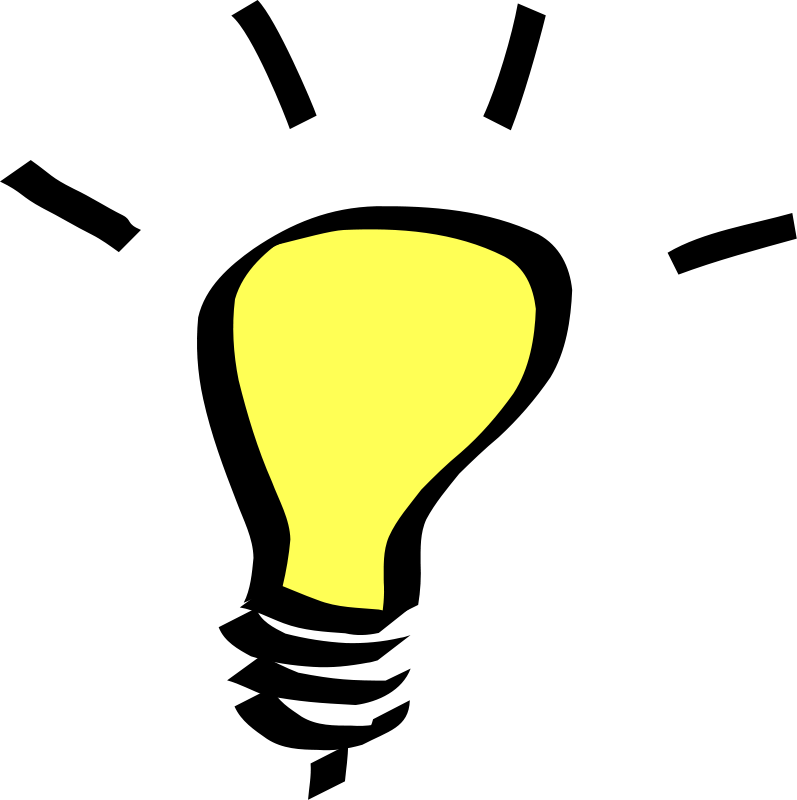
\includegraphics[height=1.1\baselineskip]{images/lamp.png}}} \underline{\textbf{Idea:}} traces back to \href{https://en.wikipedia.org/wiki/Eugene_Wigner}{Wigner} (1959). Experimentally, we can measure and control \textbf{transition probabilities}\index{Transition probabilities}\marginnote{So the physics tells us that this is something relevant}: let us represent the pure states by the rank-1 orthogonal projectors \[
P_{\psi}=|\psi\rangle\langle\psi|\qquad P_{\phi}=|\phi\rangle\langle\phi|
\]
The transition probability is defined as:
\[
\text{Prob}([\phi],[\psi]):=\Tr(P_{\psi}P_{\phi})={\color{red}|\langle\psi|\phi\rangle|^2}
\]
The relevant physical information is not the inner product, but its modulus $\Rightarrow$ \underline{\textbf{Moral:}} {\color{red}$|\langle\psi|\phi\rangle|$ should be preserved!}. The physicists' and geometers' viewpoints agree.

\underline{\textbf{Hp:}} $\mathcal{H}$ is a complex, separable Hilbert space (with finite or infinite dimension).
\begin{definition}[Projective automorphism]\index{Projective automorphism}
A projective automorphism of $\mathbb{P}\mathcal{H}$ is a map $\hat{T}:\mathbb{P}\mathcal{H}\xrightarrow[]{}\mathbb{P}\mathcal{H}$ which:
\begin{enumerate}
    \item is bijective
    \item preserves the \textbf{pseudo-angle}\index{Pseudo-angle}:
    \[
    P([\psi],[\varphi]):=\frac{|\langle\psi|\varphi\rangle|}{\lVert\psi\rVert\lVert\varphi\rVert}
    \]
    In the sense that $P(\hat{T}[\psi],\hat{T}[\varphi])=P([\psi],[\varphi]) \ \forall\;\varphi,\psi\neq 0$. The \textbf{modulus} gives independence on the representative.
\end{enumerate}
\end{definition}
Suppose to have:
\[
\begin{cases}[\psi]=[e^{i\eta}\psi]\\
[\varphi]=[e^{i\theta}\varphi]
\end{cases}\xrightarrow[]{}|\langle e^{i\eta}\psi|e^{i\theta}\varphi\rangle|=|\langle\psi|\varphi\rangle|
\]
{\fontencoding{U}\fontfamily{futs}\selectfont\char 66\relax}Two vectors define the \textbf{same ray!} The main point is that the \textbf{pseudo-angle} is independent on the \textbf{representative vector}.
\begin{example}
Projective automorphisms induced by \textbf{unitary operators:\marginnote{This is a very large source of projective automorphisms.}} let $U\in\pazocal{U}(\mathcal{H})$, then we can define $\hat{T}_U:\mathbb{P}\mathcal{H}\xrightarrow[]{}\mathbb{P}\mathcal{H}$ as {\color{red}$\hat{T}_U[\psi]=[U\psi]$}, this is a projective automorphism. The unitary operator preserves the inner product therefore it preserves the pseudo-angle. 
\end{example}
For the next example, we first have to define what is an \textbf{anti-unitary operator}.
\begin{definition}[Anti-unitary operator]\index{Anti-unitary operator}
An anti-unitary operator is a map $\Theta:\mathcal{H}\xrightarrow[]{}\mathcal{H}$ which is:
\begin{enumerate}
    \item \textbf{anti-linear:}\marginnote{This is linear over the real numbers. With $\overline{\lambda}$ we indicate the complex conjugate} $\Theta(\lambda\psi)=\overline{\lambda}\Theta(\psi)$
    \item $\langle\Theta\psi|\Theta\varphi\rangle=\overline{\langle\psi|\varphi\rangle}\overset{\mathclap{\tikz \node {$\downarrow$} node [above=1.25ex] {\footnotesize by hermitianity};}}{=}\langle\varphi|\psi\rangle$, in particular, it implies that the norm is preserved $\Rightarrow\lVert\Theta\psi\rVert=\lVert\psi\rVert$, hence it is \textbf{injective}
    \item $\Theta$ is \textbf{surjective} \marginnote{3) is a consequence of the two above if the Hilbert space is finite dimensional}
\end{enumerate}
\end{definition}
\begin{example}
Projective automorphisms induced by \textbf{anti-unitary operators:} let $\mathcal{H}=L^2(\mathbb{R}^d,dx)\ni\psi$. We define \[
(\Theta\psi)(x)=\overline{\psi(x)} \quad (\textrm{complex conjugation})
\]
\end{example}
Notice that an abstract Hilbert space has no complex conjugation because it might depend on the basis, if we introduce an ortho-normal basis and take the complex conjugate of all the components it is okay but if we change basis we will have something else. In order to have a complex conjugation we need an additional structure, for example we need to know that the Hilbert space is a space of functions.

Let $\Theta$ be an anti-unitary operator, then we can define \[
{\color{red}\hat{T}_{\Theta}[\psi]:=[\Theta\psi]}
\]which is a \textbf{projective automorphism} (check it alone).

We have two families of examples which allow us to generate projective automorphisms by using either unitary or anti-unitary operator. The good news is that these two families represent all the possible ways in which we can generate projective automorphisms.\marginnote{We are considering $\mathcal{H}$ a complex separable Hilbert space, arbitrary dimension}
\begin{theorem}[Wigner]\index{Wigner}
\labthm{Wigner}
Every \textbf{projective automorphism} in $\mathcal{H}$ is either induced by a \textbf{unitary operator} or by an \textbf{anti-unitary operator}. (\textit{No other cases)}
\end{theorem}
The inducing unitary or anti-unitary operator is \textbf{unique up to a phase}, i.e.
\[
\hat{T}_U=\hat{T}_{\eta U} \quad \textrm{for }\eta\in\textrm{U}(1)
\]
In the practice, we will encounter very very often unitary operators and not so often anti-unitary operators, but there is a case in which by fundamental reasons\marginnote{Fundamental reasons that we have no time to explain} we need anti-unitary operators: \textbf{time reversal symmetry}.

We did not decide a-priori which structure of the state space should be preserved but we let experiments tell us what is the relevant structure. If we had been able to measure and control the inner product of states without the modulus, we could have defined automorphisms in a stronger sense, requiring them to preserve the real angle and not only the pseudo-angle. But this is not possible, since as far as we know we can control transition probabilities but not the true angle, therefore this is the good physical relevant notion of automorphisms.
\section{Projective representation of groups}
It is a fact of life that transformations do not come alone, they come in groups\marginnote{Originally the word \textit{group} was an informal one but now after 100 years it took a technical sense.}. We have to represent groups in terms of projective transformations, we will be mainly interested in Lie groups but not only them. 

\underline{\textbf{Remark:}} we denote by Aut($\mathbb{P}\mathcal{H})$ the set of all projective automorphisms. Then $
\big(\textrm{Aut}(\mathbb{P}\mathcal{H}),\circ\big)$ is a group, it can be checked that the composition $\hat{T}_1\circ\hat{T}_2$ preserves the pseudo-angle. 
\begin{definition}[Projective representation]\index{Projective representation}
Let $G$ be a (physically relevant\marginnote{Physically relevant i.e. rotations, translations, Poincaré, $\dots$}) group. A \textbf{projective representation of $G$} is a \textbf{homomorphism}:
\begin{align*}
    G&\xrightarrow[]{{\text{hom}}}\text{Aut}(\mathbb{P}\mathcal{H})\\
    g&\mapsto \hat{T}_g
\end{align*}
Namely:
\begin{equation}\labeq{def-prof-rep}
(\star) \quad \hat{T}_{gh}=\hat{T}_g\circ\hat{T}_h \quad \forall g,h\in G
\end{equation}
\end{definition}
This is dictated from physics, we decided that the relevant structure is the one of transition probabilities so the automorphisms we are interested in are projective automorphisms. Now we want that our group, say the rotation groups, is represented in terms of projective automorphisms. By Wigner \refthm{Wigner}, we know that $\hat{T}_g=\hat{T}_{\color{red}U_g}$, where $U$ is a \textbf{unitary} or \textbf{anti-unitary} operator\marginnote{For simplicity, forget about anti-unitary operators for the moment}. Notice that $U_g$ is not unique: if we take 
\[
\Tilde{U}_g=\eta(g)U_g \quad \eta(g)\in\textrm{U}(1)
\]
(so with $\eta(g)$ a uni-modular number), these two guys induce the same projective automorphism $\hat{T}_{U_g}=\hat{T}_{\Tilde{U}_g}$. What do we have to require to the unitary operator in order to satisfy the condition (\ref{eq:def-prof-rep})?
\begin{equation}\labeq{cond-unit-rep}
{\color{red}U_{gh}=\omega(g,h)U_gU_h \quad \Big|\Big| \quad \star}
\end{equation}
with $\omega(g,h)\in\textrm{U}(1)$. We are interested in maps from the (physically relevant) group to the group of unitary operators which preserve the product up to a phase.
\begin{definition}[Projective unitary representation]\index{Projective unitary representation}\labdef{Projective unitary representation}
A map:\marginnote{$\pazocal{U}(\mathcal{H})$ is the group of unitary operators}
\begin{align*}
    G&\xrightarrow[]{}\pazocal{U}(\mathcal{H})\\
    g&\mapsto U_g
\end{align*}
which satisfies (\ref{eq:cond-unit-rep}) is called a \textbf{projective unitary representation} of $G$ in $\mathcal{H}$.
\end{definition}
Here the terminology is a bit odd because a projective unitary representation is not a unitary representation because a unitary representation would satisfy (\ref{eq:cond-unit-rep}) with a phase identically equal to one but the people who chose this terminology did it wrongly. The \refdef{Projective unitary representation} above contrasts with:
\begin{definition}
A (true) \textbf{unitary representation} of $G$ in $\mathcal{H}$ is a map $G\xrightarrow[]{{\color{red}hom}}\pazocal{U}(\mathcal{H})$. Namely
\begin{equation}\labeq{true-cond-unit-rep}
(\star\star) \quad U_{gh}=U_gU_h \quad \forall g,h \in G
\end{equation}
\end{definition}
\begin{kaobox}[frametitle=Remark]
It is clear that the condition (\ref{eq:true-cond-unit-rep}) is \textbf{stronger} than the condition (\ref{eq:cond-unit-rep}), so not every projective unitary representation is a true projective unitary representation.
\end{kaobox}
Here the terminology is misleading but this happens in mathematics, for example the cylindrical measure is not a measure. Now there is a very natural question: $U$ is defined up to a phase so we can choose the phase in a way to cancel out the $\omega(g,h)$ in (\ref{eq:cond-unit-rep}). Is it always possible to promote a projective unitary representation to a true projective unitary representation?
%Fine seconda parte lezione 20 (13/05/2022)
%INIZIO LEZIONE 21 19/05/2022
\section{Fundamental questions}
Given a projective unitary representation $g\mapsto U_g$, we can \textbf{\textit{readjust} (Read)} it\marginnote{This is equivalent of a change of gauge in the electromagnetic theory} by setting
\begin{equation}\labeq{read}
(\textrm{Read})\quad \Tilde{U}_g=\eta(g)U_g \quad \textrm{for } \ \eta(g)\in\textrm{U}(1), \quad \forall\;g\in G
\end{equation}
by exploiting the fact that $\hat{T}_{\eta U}=\hat{T}_U$. The map $g\mapsto\Tilde{U}_g$ will still satisfy (\ref{eq:cond-unit-rep}), but with a different phase factor $\Tilde{\omega}:$\marginnote{$U_{gh}=\omega(g,h)U_gU_h\quad$ (\ref{eq:cond-unit-rep})

Eq = Equivalence}
\begin{equation}\labeq{equivalence}
{\color{red}\Tilde{\omega}(g,h)=\eta(gh)\omega(g,h)\eta(g)^{-1}\eta(h)^{-1}} \quad (\textrm{Eq})
\end{equation}
\underline{Detail:} 
\[
\begin{split}
\Tilde{U}_{gh}&=\eta(gh)U_{gh}\overset{(\ref{eq:cond-unit-rep})}{=}\eta(gh)\omega(g,h)U_gU_h\overset{\mathclap{\tikz \node {$\downarrow$} node [above=1.25ex] {\footnotesize read (\ref{eq:read}) the other way around};}}{=}\underbrace{\eta(gh)\omega(g,h)\eta(g)^{-1}\eta(h)^{-1}}_{\Tilde{\omega}(g,h)}\Tilde{U}_g\Tilde{U}_h
\end{split}
\]
If it happens\marginnote{It depends on many things: the group, the representation etc...} that $\Tilde{\omega}(g,h)\equiv 1$, then it means that the \textbf{projective unitary representation} is equivalent via readjustment (\ref{eq:read}) to a (\textit{true}) unitary representation.

\textbf{Fundamental question}: given a projective unitary representation
\[
G\ni g \mapsto U_g\in\pazocal{U}(\mathcal{H})
\]
is it possible to \textit{\textbf{readjust}} it to obtain a (\textit{true}) unitary representation?

Before answering this question, let us state a more general question. Notice that the \textbf{factor}
\begin{align*}
    \omega:G\times G&\xrightarrow[]{}\text{U}(1)\\
    (g,h)&\mapsto\omega(g,h)
\end{align*}
must satisfy some \underline{\textbf{constraints}}:
\begin{enumerate}
    \item Associativity: since $(gh)l=g(hl) \ \forall\;g,h,l\in G$, with a little computation, one has
    \[
    \omega(g,h)\omega(gh,l)=\omega(h,l)\omega(g,hl)
    \]
    \item Normalization: if we ask that $U_e=\mathbb{1}$ [always possible]\marginnote{There is a little lemma which guarantees us that, which we omitted}, then $\omega$ should satisfy
    \[
    \omega(g,e)=1=\omega(e,g)
    \]
\end{enumerate}
\begin{exercise}
Set $\omega\sim\Tilde{\omega}$ if $\exists\;\eta:G\to\textrm{U}(1)$ such that \refeq{equivalence} is satisfied. Check that $\omega\sim\Tilde{\omega}$ is an \textbf{equivalence relation} on the set
\begin{equation}\labeq{set-eq-rel}
\Omega:=\Bqty{\omega:G\times G\to\textrm{U}(1): \textrm{1. and 2. are satisfied}}
\end{equation}
\end{exercise}
\textbf{General question:} given a group $G$, \textbf{classify all the equivalence classes} of phase factors in the set $\Omega$ defined in \refeq{set-eq-rel}.
\section{Some answers (not the most general)}\marginnote{The professor decided not to give the most general answer, because it would be too technical}
\subsection{Bargmann theory}
\begin{marginfigure}
	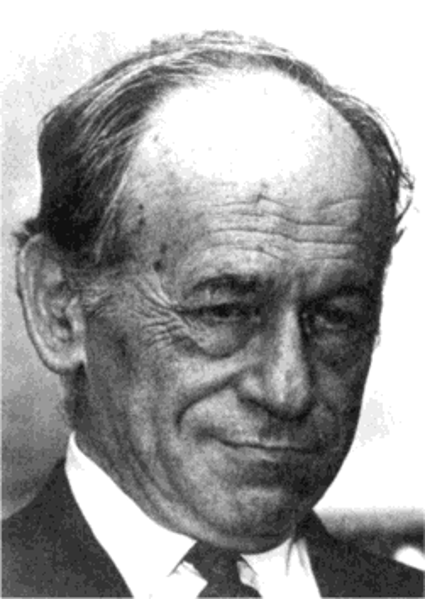
\includegraphics[width=1\linewidth]{images/Bargmann.png}
	\caption[Photo of Bargmann]{From \href{https://en.wikipedia.org/wiki/Valentine_Bargmann}{Wikipedia}: Valentine "Valya" Bargmann (April 6, 1908 – July 20, 1989) was a German-American mathematician and theoretical physicist. Born in Berlin, Germany, to a German Jewish family, Bargmann studied there from 1925 to 1933. After the National Socialist Machtergreifung, he moved to Switzerland to the University of Zürich where he received his Ph.D. under Gregor Wentzel. He emigrated to the U.S., barely managing immigration acceptance as his German passport was to be revoked—with only two days of validity left. Bargmann's theorem (1954) on projective unitary representations of Lie groups gives a condition for when a projective unitary representation of a Lie group comes from an ordinary unitary representation of its universal cover. }
	\labfig{Bargmann}
\end{marginfigure}
The \href{https://en.wikipedia.org/wiki/Projective_representation\#Infinite-dimensional_projective_unitary_representations:_Bargmann's_theorem}{following theorem} is a milestone in the chapter of group theory in quantum mechanics.
\begin{theorem}[{Bargmann, Ann. Math. 1959}]
\labthm{bargmann}\index{Bargmann theorem}
Let $G$ be a Lie group. Suppose that $G$ is (\textbf{connected}), \textbf{simply-connected}\footnote{In our version of simply connectedness is already included the connectedness.} (global properties) and \textbf{semi-simple} [local property, condition on Lie algebra]. Then \underline{every} projective unitary representation of $G$ is equivalent to a (\underline{true}) unitary representation.
\end{theorem}
Before explaining what \textit{semi-simple} means, let us see some examples.
\begin{example}
Let $G=\textrm{SU}(2)$. It is a very important example both for the theory of angular momentum and for electroweak theory, since we do not have to care about phases.
\end{example}
\begin{example}
Suppose to choose some universal covering group $\Tilde{G}$, which is simply connected by definition, of some \textbf{semi-simple} $G$ (the only requirement that we cannot avoid). In this case we have that the theorem holds true for $\Tilde{G}$, not for $G$.
\end{example}
\tetxbf{\underline{Question}:} What does \textbf{semi-simple} mean?\index{Semi-simple algebra}

\underline{Hp:} Suppose $\mathfrak{g}$ is a Lie algebra, we define:
\begin{definition}[Subalgebra, ideal - ideale]\index{Subalgebra}\index{Idea} A \textbf{subalgebra} $\mathfrak{h}$ is a subset $\mathfrak{h}\subseteq\mathfrak{g}$ such that:
\renewcommand{\labelenumi}{\Roman{enumi})}
\begin{enumerate}
    \item $\mathfrak{h}$ is a \textbf{linear subspace} of $\mathfrak{g}$
    \item $\forall\;H_1,H_2\in\mathfrak{h}\quad \comm{H_1}{H_2}\in\mathfrak{h}$ 
\end{enumerate}
A subalgebra $\mathfrak{h}\leq\mathfrak{g}$ is an \textbf{ideal} if additionally
\renewcommand{\labelenumi}{III)}
\begin{enumerate}
    \item $\forall\;H\in\mathfrak{h}, \ \forall\;X\in\mathfrak{g}\quad \comm{H}{X}\in\mathfrak{h}$
\end{enumerate}
\end{definition}
Notice that there is a parallel (an analogy):
\begin{table}[H]
    \centering
    \begin{tabular}{c|c}
        Group & Algebra\\
        Subgroup & Subalgebra\\ 
        \textbf{Normal} subgroup & \textbf{ideal}\\
        $\mathbf{N}\trianglelefteq\mathbf{G}$ & $\mathfrak{n}\trianglelefteq\mathfrak{g}$ \\
        \( \nicefrac{\displaystyle\mathbf{G}}{\displaystyle\mathbf{N}}\) \textbf{is a group} & \(\nicefrac{\displaystyle\mathfrak{g}}{\displaystyle\mathfrak{n}}\) \textbf{is a Lie algebra}
        \end{tabular}
    \caption{Analogy between subgroup and subalgebra}
    \label{tab:analogy}
\end{table}
\underline{\textbf{Reduction:}}\index{Reduction} if $\mathfrak{n}\trianglelefteq\mathfrak{g}$, we can \textit{reduce} $\mathfrak{g}$
\[
\nicefrac{\displaystyle\mathfrak{g}}{\displaystyle\mathfrak{n}}\ \textrm{ is a new object}
\]
So now it is very natural to say if a Lie algebra is irreducible.
\begin{definition}[Irreducible Lie algebra]\labdef{Irreducible-Lie-algebra}\index{Irreducible Lie algebra}A Lie algebra $\mathfrak{g}$ is \textbf{irreducible} if it does not contain any ideal except the trivial ones, i.e. $\{0\}$ and $\mathfrak{g}$.
\end{definition}
\begin{definition}[Simple Lie algebra]\index{Simple Lie algebra}
A Lie algebra $\mathfrak{g}$ is \underline{\textbf{simple}} if it is \textbf{irreducible} and $\dim\mathfrak{g}\geq 2$.
\end{definition}
\begin{proposition}\labprop{sl2-simple}
The Lie algebra $\mathfrak{sl}(2;\mathbb{C})$ is simple.
\end{proposition}
\begin{exercise}
Prove \refprop{sl2-simple}.\marginnote{Solution from page 53, in the book by Hall \cite{Hall2015_Ch3}}

\underline{Hint:} This Lie algebra has dimension 6 over the reals, but then it has dimension 3 over the complexes. Over the complex $\mathbb{C}$, use the basis
\[
X=\mqty(\admat[0]{1,0}) \qquad Y=\mqty(\admat[0]{0,1}) \qquad H=\mqty(\dmat[0]{1,-1})
\]
Suppose that there is an ideal $\mathfrak{h}\trianglelefteq\mathfrak{sl}(2,\mathbb{C})$ and that it contains the element
\[
Z=aX+bH+cY
\]
Prove that either $\mathfrak{h}=\{0\}$ or $\mathfrak{h}=\mathfrak{sl}(2,\mathbb{C})$.
\end{exercise}
\begin{proof}
Solution from page 53, in the book by Hall \sidecite{Hall2015_Ch3}. Direct calculation shows that these basis elements have the following commutation relations: $\comm{X}{Y}=H$, $\comm{H}{X}=2X$, and $\comm{H}{Y}=-2Y$. Suppose $\mathfrak{h}$ is an ideal in $\mathfrak{sl}(2;\mathbb{C})$ and that $\mathfrak{h}$ contains an element $Z=aX+bH+cY$, where $a,b$, and $c$ are not all zero. We will show, then, that $\mathfrak{h}=\mathfrak{sl}(2;\mathbb{C})$. Suppose first that $c\neq 0$. Then the element
\[
\comm{X}{\comm{X}{Z}}=\comm{X}{[-2bX+cH]}=-2cX
\]
is a nonzero multiple of $X$. Since $\mathfrak{h}$ is an ideal, we conclude that $X\in\mathfrak{h}$. But $\comm{Y}{X}$ is a nonzero multiple of $H$ and $\comm{Y}{\comm{Y}{X}}$ is a nonzero multiple of $Y$, showing that $Y$ and $H$ also belong to $\mathfrak{h}$, from which we conclude that $\mathfrak{h}=\mathfrak{sl}(2;\mathbb{C})$.

Suppose next that $c=0$ but $b\neq 0$. Then $\comm{X}{Z}$ is a nonzero multiple of $X$ and we may then apply the same argument in the previous paragraph [of Hall ndr.] to show that $\mathfrak{h}=\mathfrak{sl}(2;\mathbb{C})$. Finally, if $c=0$ and $b=0$ but $a\neq 0$, then $Z$ itself is a nonzero multiple of $X$ and we again conclude that $\mathfrak{h}=\mathfrak{sl}(2;\mathbb{C})$.
\end{proof}
\begin{definition}[Semi-simple Lie algebra]\index{Semi-simple Lie algebra}A Lie algebra $\mathfrak{g}$ is called \textbf{semi-simple} if it is:
\[
\mathfrak{g}=\bigoplus_{j=1}^N\mathfrak{s}_i
\]
with $\mathfrak{s}_i$ simple Lie algebras.
\end{definition}
\begin{kaobox}[frametitle=Remark]
Notice that the direct sum of Lie algebras is not only the direct sum of vector spaces, we ask them that they are algebraically independent and not only linear independent. Direct sum means
\[
\comm{X}{Y}=0\quad \begin{cases}
X\in\mathfrak{s}_j&\\
&j\neq l\\
Y\in\mathfrak{s}_l&
\end{cases}
\]
\end{kaobox}
{\fontencoding{U}\fontfamily{futs}\selectfont\char 66\relax} Caveat: Bargmann theorem is a sufficient condition, but \textbf{not necessary}.\marginnote{There might be a group which is not simply connected, but nevertheless its magic property holds true}

There is actually a relevant example: the \textbf{Lorentz} and \textbf{Poincaré} groups are not simply connected, but they have the \textit{magic property}.

\textbf{Bad boy:} $\textrm{SO}(3)$. As it is not simply connected, the Bargmann \refthm{bargmann} does not hold true. But then it comes another piece, which is the univeral covering: $\textrm{SO}(3)$ is a bad boy, but it has a brother which is a good boy and we can use the universal covering to simplify the picture.
\subsection{Universal covering}
\begin{marginfigure}
	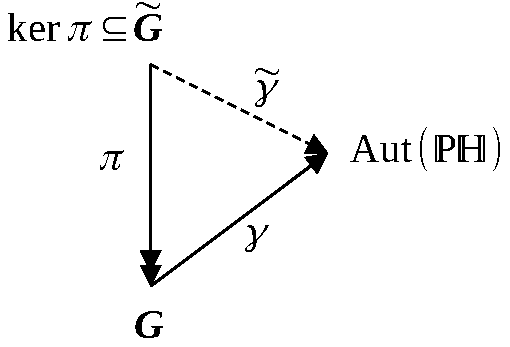
\includegraphics[width=1.1\linewidth]{images/teorem_universal_covering.pdf}
	\caption*{}
	\labfig{univ-cov}
\end{marginfigure}
\begin{theorem}
Let $G$ be a connected Lie group, and $\Tilde{G}$ its universal covering. We know that there is a Lie group homomorphism $\pi$ which is surjective and in which the number of pre-images is constant, we also know that we can describe $\Tilde{G}$ using the kernel of $\pi$
\[
\ker\pi=\left\{g\in\Tilde{G}:\pi(g)=e_{G}\right\}
\]
and that $G$ can be recovered simply by taking the quotient
\[
G=\nicefrac{\displaystyle\Tilde{G}}{\displaystyle\ker\pi}
\]
Then every projective representation $\gamma:G\to\textrm{Aut}(\mathbb{P}\mathcal{H})$ is obtained by a projective representation
\[
\Tilde{\gamma}:\Tilde{G}\to\textrm{Aut}(\mathbb{P}\mathcal{H})\quad \textrm{such that}\quad \ker\pi\subseteq\ker\Tilde{\gamma}
\]
\end{theorem}
This is a nice theorem and the prototype example is the following:
\begin{marginfigure}
	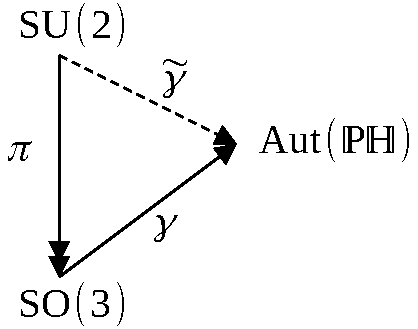
\includegraphics[width=1.1\linewidth]{images/ex_teorem_universal_covering.pdf}
	\caption*{}
	\labfig{ex-univ-cov}
\end{marginfigure}
\begin{example}
$\textrm{SU}(2)$ is the universal covering of $\textrm{SO}(3)$, it is surjective and the kernel is $\pm$ the identity
\[
\ker\pi=\left\{\pm\mathbb{1}\right\}
\]
Quantum theory tells us that we should investigate the projective representation of $\textrm{SO}(3)$, because the transformation in physical space is given by rotations, not by elements of $\textrm{SU}(2)$. So we should study maps $\gamma$ from $\textrm{SO}(3)$ to the automorphism of the projective Hilbert space $\textrm{Aut}(\mathbb{P}\mathcal{H})$.

This would be difficult because these ones are projective unitary representations, so the phase cannot be eliminated. But now we go upstairs to the universal covering and we study all the projective unitary representation of $\textrm{SU}(2)$. Since $\textrm{SU}(2)$ is a good group (it satisfies the assumption of Bargamann theorem), the projective unitary representations of $\textrm{SU}(2)$ are the true unitary representations of $\textrm{SU}(2)$. 

We study all of them, we look at the kernel and, if the kernel contains the kernel of $\pi$, then this representation will be also a representation of the group downstairs (the rotation group), otherwise it will not.
\end{example}
Now we understand that \textit{our} book in elementary quantum mechanics was not cheating, was simply a bit sloppy in explaining these facts.
\subsection{Solution to the general problem (outlook)}\marginnote{\textit{outlook} means that we just give a vague idea and it will be not asked at the exam except for \textit{cum laude}}
We have this general problem and the idea is that it can be broken in two subproblems:
\[
\textrm{Problem}\;\to\ \begin{cases}
\textrm{local}\ &\to \text{\parbox{5 cm}{\centering classify factors $\omega$ of local representations (\textbf{Lie algebras})}}\\
&\\
\textrm{global}\ &\to \text{\parbox{5 cm}{\centering which factors can be globally extended}}
\end{cases}
\]
\subsubsection{Local problem}
The local problem is done like the following.
\begin{enumerate}
    \item Within each equivalence class $[\omega]$ of factors, it is always possible to find a factor (hence a map $g\mapsto U_g$) such that \textbf{one-parameter subgroups} give \textbf{unitary representations}. Let us represent it in a diagram
    \[
    \begin{aligned}
    \mathbb{R}&\xrightarrow[]{\textrm{hom}}\mathbf{G}\overset{\mathclap{\tikz \node {$\downarrow$} node [above=1.25ex] {\footnotesize Not a homomorphism, because of $\omega$ (because of the phase)};}}{\to} \pazocal{U}(\mathcal{H})\\
    t&\mapsto g(t)\mapsto U_{g(t)}\equiv U_t
    \end{aligned}
    \]
    such that $g(t+s)=g(t)g(s)$ (it is also implied that $g(0)$ is the neutral element of the group). In a sense, we look at our projective unitary representation along a one-dimensional subgroup, and it happens that along this subgroup, we do not need the phase: $U_{t+s}=1\cdot U_tU_s$
    \item Moreover we check that the map $t\mapsto U_t$ is \textbf{strongly continuous}\marginnote{we specify in which sense is continuos since our Hilbert space might be infinite dimensional}:
    \[
    \forall\;\psi\in\mathcal{H},\;\forall\;t\in\mathbb{R}\quad \lim_{h\to 0}U(t+h)\psi=U(t)\psi
    \]
    In view of the group property we can check it just at $t=0$ and then it will be true for all times.
    \begin{figure}[h!]
	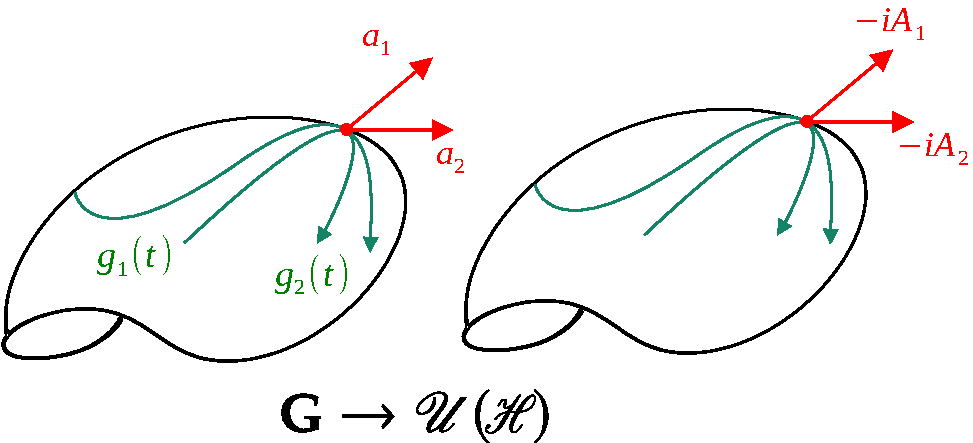
\includegraphics[width=1\linewidth]{images/local_problem.pdf}
	\caption{Lie group and map to the unitary group.}
	\labfig{loc-prob}
    \end{figure}
    Then there is an important mathematical-quantum theorem which tells us that every strongly continuous one-parameter unitary group is written as the exponential of some generator: so, by \textbf{Stone theorem}\index{Stone theorem},\marginnote[-14mm]{Dal capitolo 9 di \cite{picasso2015lezioni}:
    
    <<Useremola seguente notazione: se il sistema si trova inizialmente, $t = 0$ per fissare le idee, in un certo stato descritto dal vettore $\ket{A}$, indicheremo questo vettore con $\ket{A,0}$ per mettere in evidenza l’istante in cui il sistema si trovanello stato $\ket{A}$. Con $\ket{A,t}$ indicheremo il vettore che descrive lo stato del sistema al generico istante $t$, se inizialmente il sistema era nello stato $\ket{A,0}$. Cioè, per effetto dell'evoluzione temporale: \[ \ket{A,0}\xrightarrow[]{\textrm{dopo un tempo $t$}}\ket{A,t} 
    \] 
    Assumiamo che 
    \[
    \ket{A,t}=U(t,0)\ket{A,0}
    \]
    dove $U(t,0)$ è un operatore \textit{lineare} e \textit{unitario}. In generale, se $U(t, t_0)$ è l'operatore di evoluzione temporale fra l’istante (iniziale) $t_0$ e l'istante $t$, e se ci limitiamo a considerare sistemi soggetti a forze \textit{indipendenti dal tempo} allora $U(t, t_0)$ dipende solo dall’intervallo $t-t_0$ e \textit{non} dall’istante iniziale $t_0$: in questo caso scriveremo
    \[
    U(t)\equiv U(t,0)
    \]
    e si ha che
    \[
    U(t_1)U(t_2)=U(t_2)U(t_1)=U(t_1+t_2)
    \]
    Se vale la precedente equazione (cioè le forze sono indipendenti dal tempo), si può dimostrare (\textbf{teorema di Stone}) che
    \[
    U(t)=e^{-iKt}
    \]
    dove $K$ \textbf{è un operatore autoaggiunto}.>>} one has $U_t=e^{-iA}$ with $A^\ast=A$, namely self-adjoint (in general unbounded and the minus at the exponential is purely convectional). 
    Then basically what happens is that we have the picture in \reffig{loc-prob}. On the left, we have our Lie group $G$, then we have a map from $G$ to the unitary group $\mathcal{H}$
    \[
    G\to\mathcal{U}(\mathcal{H})
    \]
    If $\mathcal{H}$ is finite-dimensional, this is still a Lie group; while if it is infinite-dimensional this will be something more general (morally we now draw it as a Lie group). We can choose several one-parameters subgroups and we know that, in a Lie group, a one-parameter subgroup is  characterized by the tangent vector: $a_1, a_2, \dots$, they will be as many as the dimension of the Lie group. Each one of them, corresponds to a one parameter subgroup: $g_1(t), g_2(t),\dots$. Via the reasoning we did before, these will correspond to one-aparameters on $\mathcal{U}(\mathcal{H})$ and they will have as generators $-iA_1,-iA_2,\dots$. Basically in doing so, we have a basis for the Lie algebra and we map it into a family of self-adjointed operators; \textbf{if} the map $g\mapsto U_g$ was a (\underline{true}) unitary representation, we would get a \textbf{faithful representation of the Lie algebra}, i.e.
    \[
    \comm{a_j}{a_l}=\sum_k{\color{red}c^k_{jl}}a_k \qquad \text{Multiplication rule in the Lie algebra}
    \]
    $c_{jl}^k$ are called \textit{the algebra structure coefficients}.
    If it were a true unitary representation, we would have that the generators satisfy the same relation\marginnote[7mm]{This is waht happens with the algebra of the angular momentum: the three operators which represent the angular momentum satisfy the same relation as the elements of the Lie lagebra $\textrm{SO}(3)$, up to an immaginary unit.}
    \WithArrowsOptions{displaystyle}
    \[
    \begin{WithArrows}
    \comm{-iA_j}{-iA_l}&=\sum_k{\color{red}c^k_{jl}}\left(-iA_k\right)\Arrow{\text{Getting rid of the "i"}}\\
    \comm{A_j}{A_l}&=i\sum_k{\color{red}c^k_{jl}}A_k
    \end{WithArrows}
    \]
    In general, $g\mapsto U_g$ is a \textbf{projective unitary representation}, and then one obtains [modernly by differentiating $\omega(g,h)$ near the identity $e$] a correction\index{Central charge}
    \[
    \comm{A_j}{A_l}=i\sum_kc^k_{jl}A_k{\color{red}\;+\underbrace{\beta_{jl}\mathbb{1}}_{\textrm{\parbox{1 cm}{\centering Central charge}}}} \qquad \Big|\Big| \quad \star
    \]
    In general one has to study what it is called a \textbf{\textit{central extension of the Lie algebra}}\index{central extension of the Lie algebra}; then we have to classify all the central extensions of the Lie algebra (it might be some work). There are some constrains:
    \begin{itemize}
        \item antysymmetry: $\beta_{lj}=-\beta_{jl}$;
        \item associativity:
        \[
        \begin{split}
        &\sum_{k=1}^d\left(c^k_{{\color{red}ij}}\beta_{{\color{red}l}k}+c^k_{{\color{red}jl}}\beta_{{\color{red}i}k}+c^k_{{\color{red}li}}\beta_{{\color{red}j}k}\right)=0\\
        &\qquad\quad {\color{red}\circlearrowleft}
        \end{split}
        \]
        where $d$ is the dimension of the Lie algebra
    \end{itemize}
    \end{enumerate}
Therefore the local problem consists in classifying all the central extensions of the Lie algebra we are interested, in hence all the matrices $\beta_{jl}$ which satisfy the constraints above.
\subsubsection{Gloabl problem}
We will not spend words on it, let us just give some

\textbf{Keywords:} Group cohomology $H^k(\mathbf{G})$
\begin{marginfigure}
	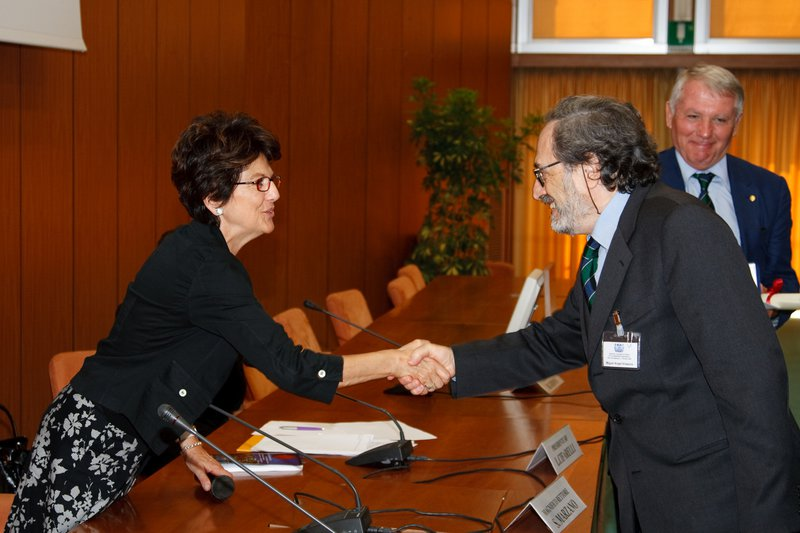
\includegraphics[width=1\linewidth]{images/virasoro.jpg}
	\caption[Virasoro at the \textit{Premio E. Fermi 2009}]{From \href{https://en.wikipedia.org/wiki/Miguel_\%C3\%81ngel_Virasoro_(physicist)}{Wikipedia}: Miguel Ángel Virasoro (Buenos Aires, 9 May 1940 – Buenos Aires, 23 July 2021) was an Argentine (naturalized Italian) theoretical physicist. Virasoro worked in Argentina, Israel, the United States, and France, but he spent most of his professional career in Italy at La Sapienza University of Rome. He shared a name with his father, the philosopher Miguel Ángel Virasoro. He was known for his foundational work in string theory, the study of spin glasses, and his research in other areas of mathematical and statistical physics. The Virasoro-Shapiro amplitude, the Virasoro algebra, the super Virasoro algebra, the Virasoro vertex operator algebra, the Virasoro group, the Virasoro conjecture, the Virasoro conformal block, and the Virasoro minimal model are all named after him. While working in Italy, Virasoro studied spin glasses and other systems in statistical mechanics. Together with Italian physicist Giorgio Parisi and French physicist Marc Mézard, Virasoro discovered the ultrametric organization of low-temperature spin glass states in infinite dimensions.}
	\labfig{Virasoro}
\end{marginfigure}
\begin{example}[\href{https://it.wikipedia.org/wiki/Algebra_di_Virasoro}{Virasoro algebra}]
We take as a group the group of diffeomorphism of the circle
\[
\mathcal{G}=\textrm{Diff}(S^1)
\]
We wrote it with this particular $G$, to remind ourselves that this is not, properly speaking, a Lie group, because it is infinite dimensional, but morally it is. Now we have its Lie algebra $\textrm{Lie}\mathcal{G}$, and then the Virasoro algebra is a \textbf{central extension of the Lie algebra to diffeomorphism} $\textrm{Lie}\textrm{Diff}(S^1)$ (actually a simple one where we just add $+c\mathbb{1}$).

There are some good reasons to study this algebra within string theory.
\end{example}
%FINE LEZIONE 21 del 19/05/2022
\end{document}